\chapter{Project 5: Game}

\section{Overview}
If you've ever owned a GameBoy or similar device, then you might be familiar with what we're going to build as part of this project.
This project will combine many of the skills from previous projects, so familiarity with those will help here. In this project you will:
\begin{itemize}
    \item Connect buttons and a screen to your microcontroller
    \item Have a basic understanding of the code that implements a basic game loop including checking for input and drawing the current frame to the screen
\end{itemize}
At the end of this project, your microcontroller should run a MicroPython program that allows you to play a very basic version of
Space Invaders. Let's get started!
\begin{figure}[H]
\centering
    \includegraphics[width=.6\linewidth]{project_5/game.jpg}
    \caption{The end result should look something like this}
\end{figure}

\pagebreak

\section{Directions}

\subsection{Creating the circuit}
Using jumper cables, you will be assembling a circuit between your microcontroller, your breadboard, and the buttons,
resistors, and OLED screen included in your kit.

\subsubsection{Remove previous components}
Before beginning, remove all components from prior chapters including the microcontroller (as we will be putting it in
a different location from the rest of the projects).

\subsubsection{Attach the microcontroller to the breadboard}
Carefully insert the pins at the bottom of your microcontroller into the breadboard. Refer back to \ref{pinout} for pin labels.
When placing the board into the breadboard, make sure that the microcontroller is oriented such that:
\begin{itemize}
    \item The pin labeled \textbf{5V} is inserted in hole at \textbf{Column H, Row 20} of the breadboard (or \textbf{H20}, for short)
    \item The pin labeled \textbf{GPIO2} is inserted in hole \textbf{D20} of the breadboard
    \item The pin labeled \textbf{GPIO20} is inserted in hole \textbf{H26} of the breadboard
    \item The pin labeled \textbf{GPIO21} is inserted in hole \textbf{D26} of the breadboard
\end{itemize}
You may need to apply more pressure than expected to seat the microcontroller properly in the breadboard. When its over, it should look like this:
\begin{figure}[H]
    \centering
    \includegraphics[width=.6\linewidth]{project_5/microcontroller_seated_in_breadboard.jpg}
    \caption{So far, so good!}
\end{figure}

\subsubsection{Connect the buttons, resistors, and the screen}
\begin{itemize}
    \item Place the OLED screen into the breadboard such that its 4 pins connect to holes \textbf{A15}, \textbf{A16}, \textbf{A17}, and \textbf{A18}.
    \item Place a button so that one connected set of pins (refer to \ref{button_basics} for an example) is in \textbf{A1}
    and \textbf{C1} and the other set is in \textbf{A3} and \textbf{C3}.
    \item Place a resistor between \textbf{E1} and the top negative rail (the blue one).
    \item Place another button so that one connected set of pins is in \textbf{A4} and \textbf{C4}
    and the other set is in \textbf{A6} and \textbf{C6}.
    \item Place a resistor between \textbf{E4} and the top negative rail.
    \item Place a third button so that one connected set of pins is in \textbf{A28} and \textbf{C28}
    and the other set is in \textbf{A30} and \textbf{C30}.
    \item Finally place a resistor between \textbf{E28} and the top negative rail.
\end{itemize}

You should be left with something that looks like this:
\begin{figure}[H]
    \centering
    \includegraphics[width=.6\linewidth]{project_5/components_placed.jpg}
    \caption{All of the components except for the jumper wires are now placed.}
\end{figure}

\subsubsection{Connect the necessary jumper wires}
\begin{itemize}
    \item Using a black jumper wire, place one end of the wire into hole \textbf{I21} of the breadboard and the other
    end in any hole on the top negative rail (the blue one). This will provide the ground connection for all of the components.
    \item Place one end of a black jumper wire between the top negative rail and hole \textbf{B15}. This will provide the ground connection
    for the OLED screen.
    \item Place one end of a red jumper wire into hole \textbf{I22} of the breadboard and the other end into
    \textbf{B16}. This will provide \textbf{3.3} volts of power to the OLED screen.
    \item Place a red jumper wire between the top positive rail and hole \textbf{B16}. This will provide power for the OLED screen.
    \item Place a white jumper wire between \textbf{B17} and \textbf{B25}. This will provide a clock signal to the OLED screen.
    \item Place a yellow jumper wire between \textbf{B18} and \textbf{B24}. This will provide the data to display on the OLED screen.
    \item Place a green jumper wire between \textbf{E3} and \textbf{B22}. This will provide the signal for the left movement.
    \item Place a green jumper wire between \textbf{E6} and \textbf{B23}. This will provide the signal for the right movement.
    \item Finally, place a purple jumper wire between \textbf{E30} and \textbf{B21}. This will provide the fire signal.
\end{itemize}

You should be left with something that looks like this:
\begin{figure}[H]
    \centering
    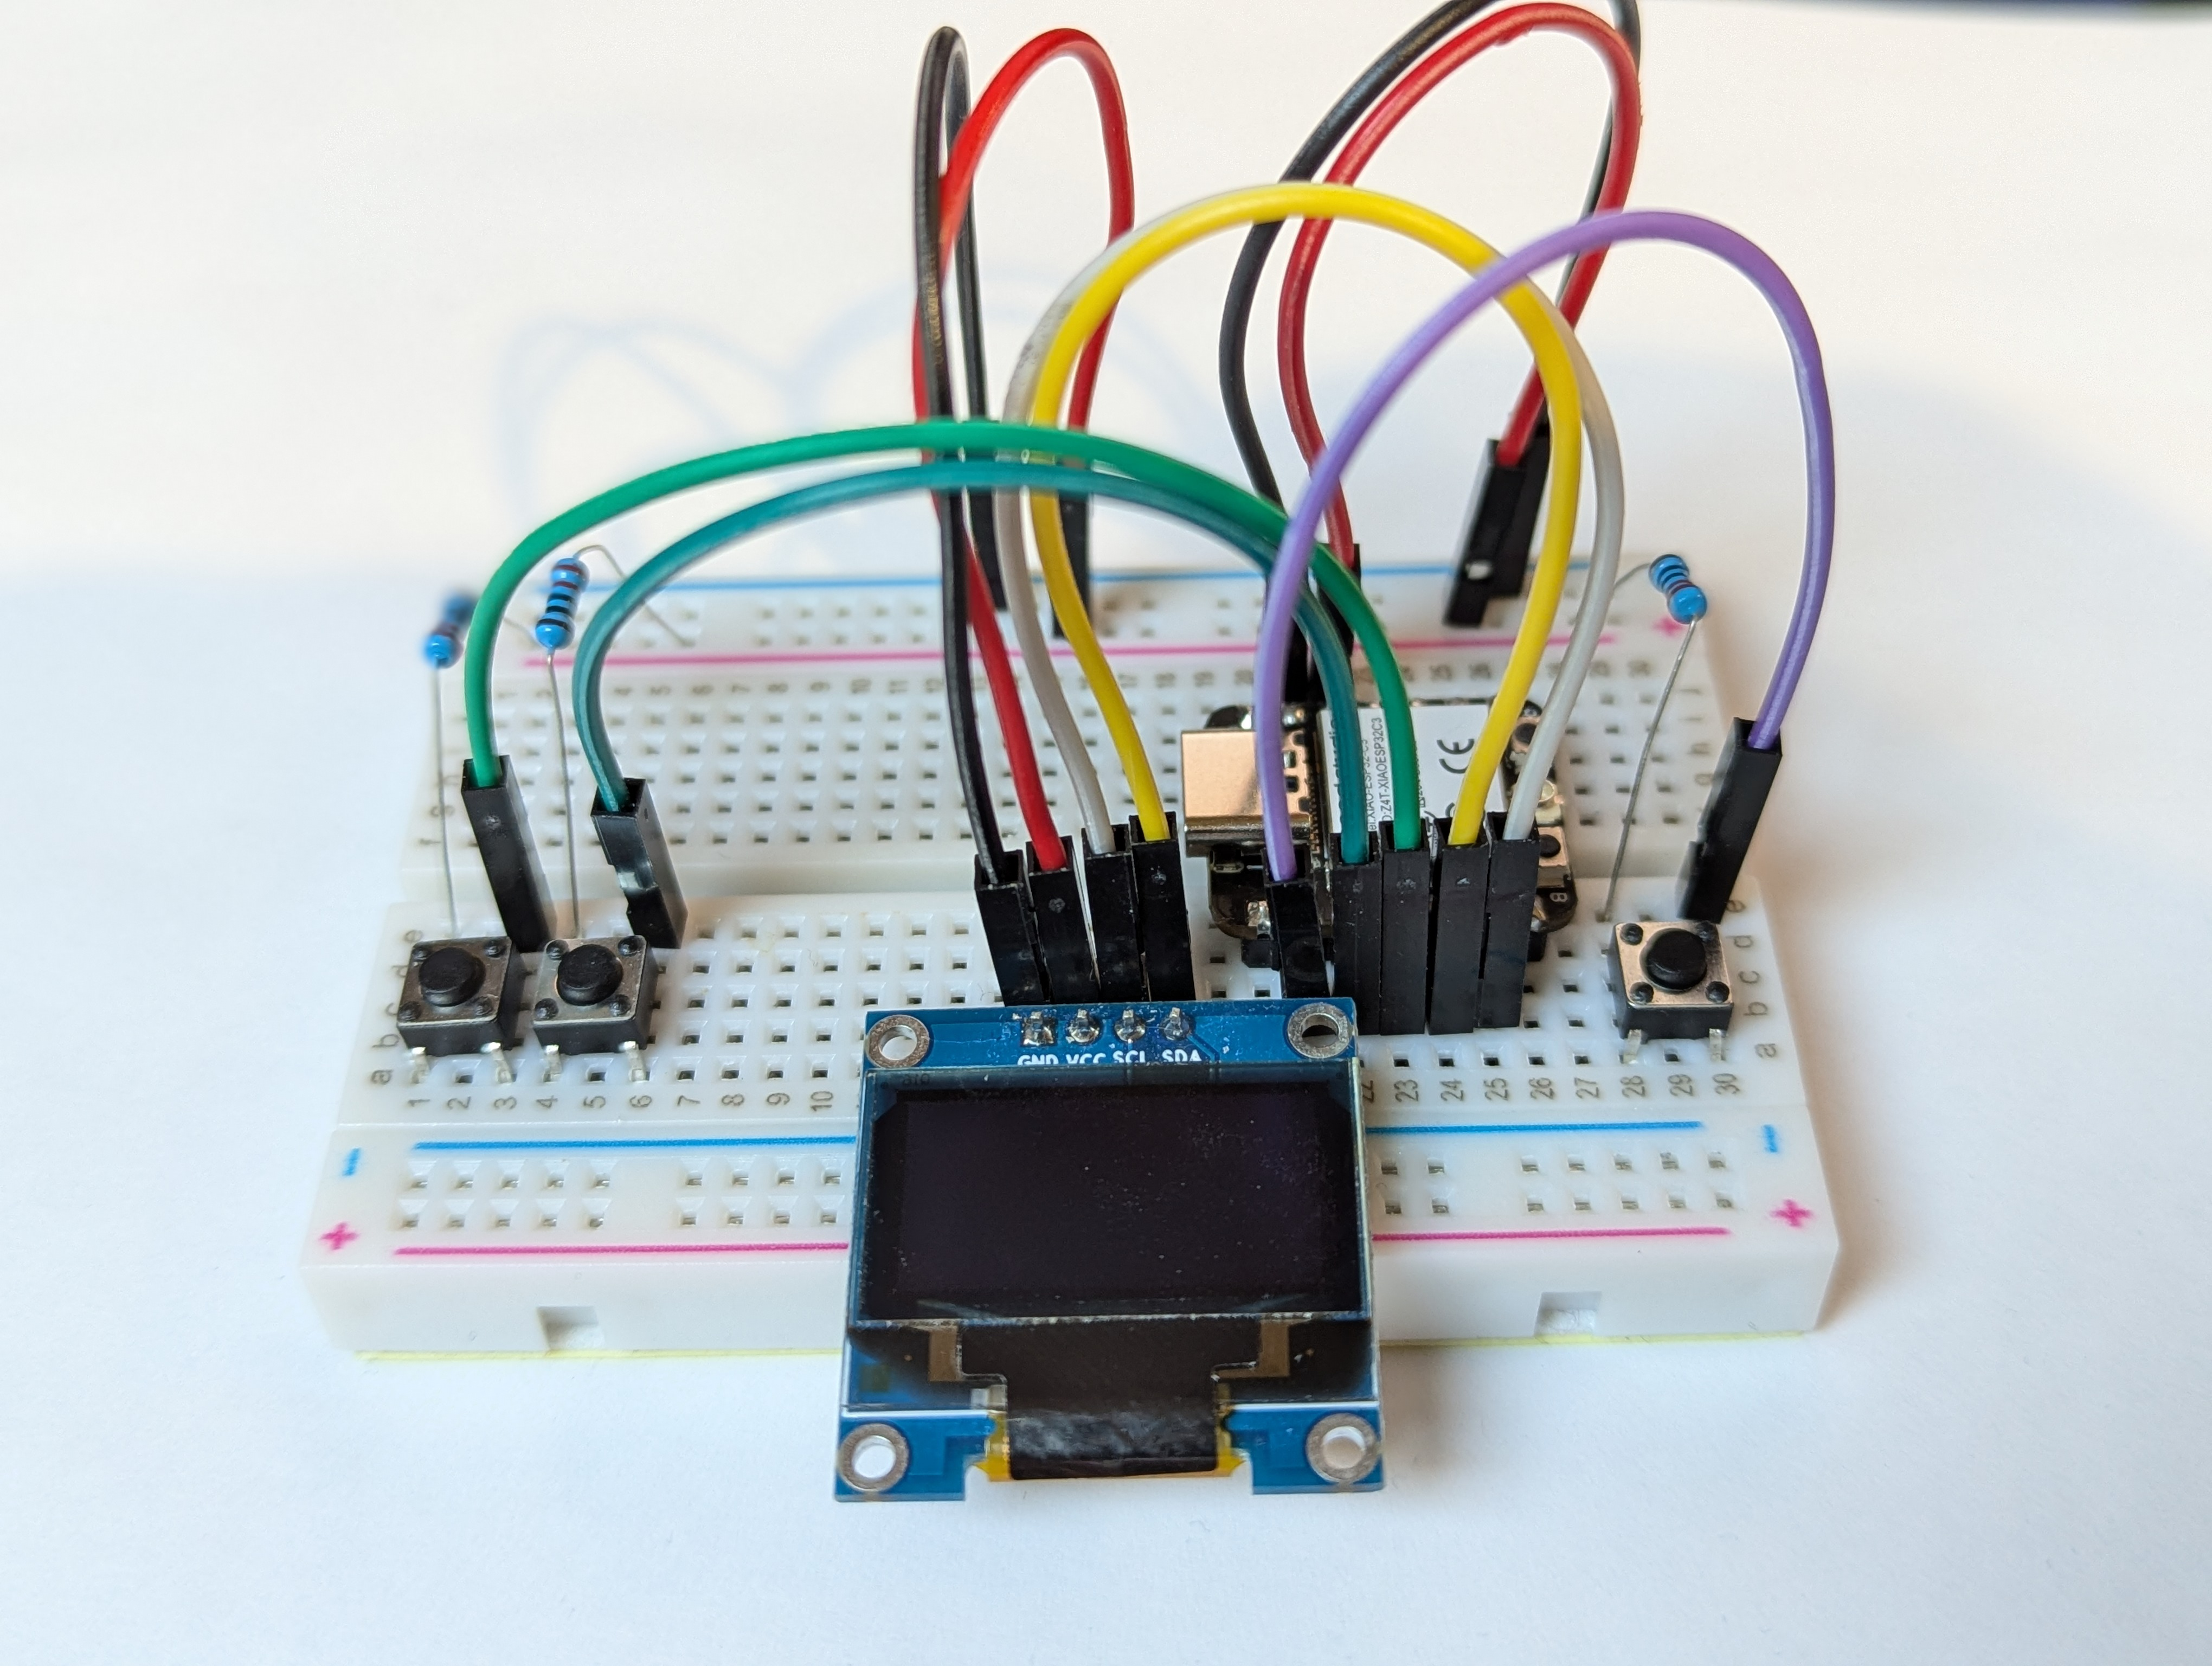
\includegraphics[width=.6\linewidth]{project_5/all_connected.jpg}
    \caption{All components and wires are now installed}
\end{figure}

\subsection{Programming the microcontroller}
Once all of the wiring is correct, connect the USB cable to the microcontroller and load the IDE to
access it. Refer back to Chapter \ref{ide} for instructions.

Click on the file named "project\_5\_game.py". This will load the code in the editor for this section. Read through the comments
and the code to get a sense for how it works. Once you are ready, you can click the blue play button in the upper left of the window
to start the game.

You can move your ship back and forth by pressing the buttons on the left. You can fire your ship's weapon by pressing the
button on the right. Once you have destroyed all of the enemy ships, a "You Win!" screen will be shown and the game will freeze.
If you want to start again, press the red stop button in the editor and then the blue play button again.

\subsection{Examining the code}

This project has the most code of any so far. The code can be broken down into several sections:
\begin{itemize}
    \item The \textbf{Missle} class
    \item The \textbf{Enemy} class
    \item The \textbf{Ship} class
    \item The \textbf{game\_loop()} function and a few helper functions (each called \textbf{update\_<x>()})
    \item A \textbf{main()} function at the bottom to get everything setup and started
\end{itemize}

Let's look at each of these below

\subsubsection{The Missle class}
\begin{lstlisting}[language=Python,caption=The Missle class]
class Missle:
"""Keeps track of an on-screen missle"""

def __init__(self, x, y):
    """Save our starting state"""
    self.x = x
    self.y = y
    self.active = True

def move(self):
    """If we move above the top of the screen, mark
    ourselves as not active. The game loop should
    cleanup any non-active missles.
    """

    global score, high_score

    self.y -= 5
    if self.y < 0:
        self.active = False

    # have we destroyed any enemies?
    for enemy in enemies:
        hitbox = enemy.hitbox
        if not hitbox[0] <= self.x <= hitbox[0] + hitbox[2]:
            continue
        if not hitbox[1] <= self.y <= hitbox[1] + hitbox[3]:
            continue
        enemy.active = False
        self.active = False
        score += 10

def draw(self):
    """Draw ourselves at our current posistion"""
    for y_offset in range(5):
        oled.pixel(self.x, self.y - y_offset, 1)
\end{lstlisting}

This class had 3 methods: an \textbf{\_\_init\_\_()} function that sets the initial state of the object,
a \textbf{move()} function that is called for each frame the missle is on screen, and a \textbf{draw()}
function which is called to tell the OLED how to display this missle.

In the \textbf{move()} function, the missle sets its position on the Y-axis upwards by 5 pixels. It then decides
if it is now higher than the top of the screen and if so, marks itself as inactive. Then it checks if it
has collided with any of the enemies that are still on the screen. If it has, it marks the enemy and
itself as destroyed and increments the player's score by 10 points.

The \textbf{draw()} function is pretty simple. It just draws a vertical line by placing 5 pixels on top of each
other, starting from the missle's current x and y coordinates.

\subsubsection{The Enemy class}
\begin{lstlisting}[language=Python,caption=The Enemy class]
class Enemy:
def __init__(self, x, y):
    self.x = x
    self.y = y
    self.active = True
    self.sprites =  [space_invaders_sprites.ENEMY_SPRITE1, space_invaders_sprites.ENEMY_SPRITE2]
    self.current_sprite = 0
    self.sprite_changed = time.ticks_ms()

@property
def hitbox(self):
    return (self.x, self.y, 16, 8)

def move(self):
    pass

def draw(self):
    now = time.ticks_ms()
    if now - self.sprite_changed > 1000:
        self.current_sprite += 1
        self.current_sprite %= len(self.sprites)
        self.sprite_changed = now
    oled.blit(self.sprites[self.current_sprite], self.x, self.y)
\end{lstlisting}

This class had 3 methods and one special method called a property. The \textbf{\_\_init\_\_()} function sets the
initial state of the object, the \textbf{move()} function that is called for each frame the enemy is on screen,
the \textbf{draw()} function is called to tell the OLED how to display this enemy. There is also a \textbf{hitbox}
property defined.

In the \textbf{\_\_init\_\_()} method, it sets some basic properties and then loads the sprite data from the external
space\_invaders\_sprites.py file. Each sprite is just an array of data that describes which pixels should be drawn
as white and which will be black. If you squint at it, you can see the shape of the enemy in the array.

The \textbf{hitbox} method is a special kind of method. It is decorated with \textbf{@property} which tells Python
to call the method and return the computed value when the property is accessed. This allows the code to dynamically
change the hitbox of the enemy if it is repositioned.

The \textbf{move()} method currently does nothing which means the enemies cannot move around the screen

The \textbf{draw()} method tells the OLED how to draw the enemy. It uses a function of the OLED library called \textbf{blit()}
which takes in the sprite data that was defined earlier and draws it to the screen in one efficient operation. This is a
much faster way that having to draw out each pixel in a loop.

\subsubsection{The Ship class}
\begin{lstlisting}[language=Python,caption=The Ship class]
class Ship:
"""Keep track of the player's ship"""

def __init__(self, x, y):
    """Save our initial state"""
    self.x = x
    self.y = y
    self.last_fired = time.ticks_ms()

def move(self):
    """Move left or right depending on which button is pressed"""

    if left_button.value() == 0:  # left pressed
        self.x -= 3
    if right_button.value() == 0:  # right pressed
        self.x += 3
    if self.x > 119:
        self.x = 119
    if self.x < 9:
        self.x = 9

def draw(self):
    """Draw the pixels of our ship"""

    oled.blit(space_invaders_sprites.SHIP_SPRITE, self.x - 8, self.y - 5)

def fire(self):
    """If the fire button is pressed and the cooldown time has
    passed, then generate a new missle object at our current position
    """

    now = time.ticks_ms()
    if fire_button.value() == 0 and now - self.last_fired > 200:
        self.last_fired = now
        missles.append(Missle(self.x, self.y - 10))
\end{lstlisting}

This class had 4 methods, the \textbf{\_\_init\_\_()} function sets the initial state of the object,
the \textbf{move()} function that is called for each frame the ship is on screen, the \textbf{draw()}
function is called to tell the OLED how to display the ship, and the \textbf{fire()} function which
checks if the fire button is pressed and creates a missle at the current ship position.

In the \textbf{move()} method, it checks if either of the left or right movement buttons are currently
pressed. If so, it moves the ship in that direction. If it detects that this ship is currently at the
edges of the screen, it doesn't move it any further.

In the \textbf{draw()} method, we use the \textbf{blit()} method mentioned previously to draw our ship's sprite to the OLED.

In the \textbf{fire()} method, we check if the fire button is currently held down. If so, it creates a new
instance of the \textbf{Missle} class and sets it's initial position to be just above the ship's current position.

\subsubsection{The game loop and helper function}
\begin{lstlisting}[language=Python,caption=The game loop and helper functions]
def update_missles():
    """Remove any non-active missles and move the rest"""

    global missles
    missles = [m for m in missles if m.active]
    for missle in missles:
        missle.move()
        missle.draw()

def update_enemies():
    """Remove any destroyed enemies and move the rest"""

    global enemies
    enemies = [e for e in enemies if e.active]
    for enemy in enemies:
        enemy.move()
        enemy.draw()

def update_score():
    global game_on
    oled.text("Score:%s" % score, 0, 0)
    if not enemies:
        oled.text("You Win!", 35, 30)
        game_on = False

def game_loop(ship):
    """Drive the main game loop"""

    oled.fill(0)
    ship.fire()
    update_missles()
    update_enemies()
    ship.move()
    ship.draw()
    update_score()
    oled.show()
\end{lstlisting}

The \textbf{game\_loop()} function is run over and over while the game is ongoing. It is responsible for
the order that all game objects are checked and redrawn. At the start of the loop it clears the entire
screen (fills all of the pixels with black). Then it checks if any new missles need to be created, updates
the existing missles, updates the enemies and the ship, and displays the current score (which also checks
if the game is over). After all objects have been updated, it tells the OLED to display everything that's
been written to it for this frame.

\subsubsection{The main function}
\begin{lstlisting}[language=Python,caption=The main function]
    def main():
    try:
        ship = Ship(64, 64)
        for y in range(12, 36, 12):
            for x in range(10, 118, 16):
                enemies.append(Enemy(x, y))
        while game_on:
            game_loop(ship)
    except KeyboardInterrupt:
        pass

main()
\end{lstlisting}

The \textbf{main()} function is pretty short, but very important. It creates instances of our ship and all
of the enemies and then runs the \textbf{game\_loop()} function over and over until the game is complete.

\section{Review}
% go over what we have accomplished (maybe go into more detail about the circuit and the pins on the microcontroller?

\section{Possible Extensions}
If you want to do some experimentation, try these:

\begin{itemize}
    \item Add some LEDs and have them light up when an enemy is hit or when the game is won.
    \item Have the enemies move around the screen. In the classic space invaders game, they moved down towards the ship as the game progressed.
\end{itemize}
